

\chapter{Casi d'Uso}                %crea il capitolo
%%%%%%%%%%%%%%%%%%%%%%%%%%%%%%%%%%%%%%%%%imposta l'intestazione di pagina
\lhead[\fancyplain{}{\bfseries\thepage}]{\fancyplain{}{\bfseries\rightmark}}
Di seguito alcuni esempi di utilizzo della libreria.
Le dimostrazioni seguenti sono state effettuate su una macchina con architettura amd64 e con installato il sistema operativo debian in versione sid (quindi unstable) ma sono state testate e riprodotte anche su altre configurazioni e distribuzioni GNU/Linux.
\section{Environment}
Come precedentemente accennato possiamo integrare la nostra libreria in vuos attraverso il modulo unrealvsnlib o creandone uno alternativo che dipenda da VSNLib.\\
\begin{description}
\item[Creazione moduli:] La creazione di un modulo \`e molto semplice e basta serguire le linee guida di quelli preesisteni, inoltre grazie ad una routine in cmake non \`e necessario aggiungere alcuna riga manualmente al makefile e sar\`a, appunto, cmake ad occuparsi della compilazione.
\item[Start Vuos:] Vuos si avvia attaverso il comando {\tt umvu} ed \`e in grado di interpretare comandi successivi come argomenti, come mostrato nell'esempio infatti {\tt umvu} \`e affiancato dal comando konsole e pertanto verr\`a lanciata una nuova istanza di terminale con ambiente vuos.
In alternativa \`e possibile utilizzare altri comandi come xterm, bash o zsh.
\item[Include dei Moduli vuos] I moduli in vuos vengono inclusi attraverso la direttiva
\begin{verbatim}
vu_insmode <nome_modulo>
\end{verbatim}
Un esempio di avvio e inclusione del modulo \`e quello della figura seguente.
\begin{figure}[h]                       %crea l'ambiente figura; [h] sta
                                        %   per here, cio� la figura va qui
\begin{center}                          %centra nel mezzo della pagina
                                        %   la figura
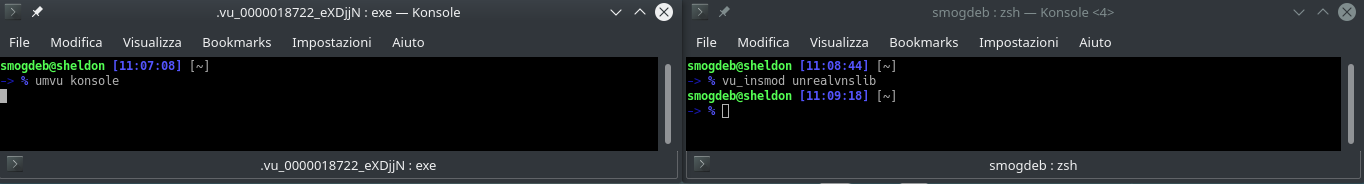
\includegraphics[width=16cm]{start_vuos}%inserisce una figura larga 5cm
                                        %se si vuole usare va scommentata
%
%%%%%%%%%%%%%%%%%%%%%%%%%%%%%%%%%%%%%%%%%inserisce la legenda ed etichetta
                                        %   la figura con \label{fig:prima}
\caption[start/include\_mod vuos]{start and include vuos}\label{fig:start_vuos}
\end{center}
\end{figure}
\end{description}
\section{Esempi}                 %crea la sezione
Nella parte successiva verr\`a mostrato un esempio di configurazione per LWIPv6 attraverso VSNLib.\\
Per semplificare la dimostrazione si \`e deciso di non utilizzare l'ambiente sopra descritto o altre tecniche di cattura delle system call ma i pacchetti netlink sono stati costruiti all'interno del codice di test. Sono esempi statici di come li creerebbe il programma \texttt{ip} ma utili a mostrare sia come \`e formato un pacchetto di questa tipologia sia per tracciare i passi compiuti per il parsing e la configurazione.
\begin{description}
\item[Init VSNLib: ]L'unico header di riferimento della libreria necessario \`e vsnshared.h, all'interno troviamo dichiarate le funzioni necessarie all'utilizzo della libreria.
\begin{lstlisting}[style=CStyle]
extern int init_vsnlib(char* stack);
extern void handle_vsnlib(void* buf, size_t len, void* nif, void* stack);
\end{lstlisting}
Come gi\`a spiegato la prima funzione serve per indicare alla libreria di quale modulo fare il load pertanto richiede come input la stringa con nome del file da caricare comprensivo di \texttt{.so} (si noti che \`e necessario specificare, tra i PATH di ricerca delle librerie, quello in cui risiede il modulo \texttt{.so}. Senza questo accorgimento il file non verr\`a trovato da dlopen provocando la terminazione del programma. La variabile dell'environment da settare \`e \texttt{LD\_LIBRARY\_PATH}, un esempio \`e mostrato in figura \ref{fig:test4}).
La seconda \`e l'unico ``handle'' per passare il pacchetto netlink che dovr\`a essere poi interpretato, inoltre prende come argomeni anche un puntatore allo stack e all'interfaccia oggetto della modifica.
\item[Strutture: ]I pacchetti netlink sono accomunati dallo stesso header, come mostrato in precedenza, ma presentano strutture diverse per il resto. In questo esempio sono stati creati i pacchetti per l'aggiunta e la rimozione di un indirizzo da un'interfaccia, l'aggiunta e la rimozione di una rotta e l'accensione/spegnimento di un'interfaccia.
\begin{lstlisting}[style=CStyle]
struct info{
  struct rtattr attr;
  unsigned char ip6_address[sizeof(struct in6_addr)];
};

  struct addr_payload{
  struct nlmsghdr header;
  struct ifaddrmsg ifa;
  struct info attribute[2];
};

struct route_payload{
  struct nlmsghdr header;
  struct rtmsg rtm;
  struct info attribute;
};

struct link_payload{
  struct nlmsghdr header;
  struct ifinfomsg ifi;
};

\end{lstlisting}
rispettivamente:
\begin{itemize}
  \item info contiene il payload con gli indirizzi.
  \item addr\_payload viene usato per aggiungere/rimuovere un indirizzo a/da un interfaccia.
  \item route\_payload usato per aggiungere/rimuovere rotte.
  \item link\_payload per attivare/disattivare l'interfaccia.
\end{itemize}
La descrizione \`e ristretta a questo esempio, ma queste strutture vengono impeigare per compiere pi\`u azioni di quelle presentate.
\item[Creazione pacchetti: ]\`E eseguita dalle funzioni nel test.
\begin{lstlisting}[style=CStyle]
void fill_buf_addr(struct link_payload* buffer, int mode, int modeIP);
void fill_buf_route(struct link_payload* buffer, int mode, int modeIP);
void fill_buf_link(struct link_payload* buffer, int mode);
\end{lstlisting}
Il compito di queste funzioni \`e riempire i campi delle strutture sopra elencate in base all'operazione richiesta, \`e possibile modificarle per ottenere comportamenti diversi e compiere altri test.\\
In pratica si occupano di fare quello che farebbe un programma come \texttt{ip} in maniera semplificata, questo rende pi\`u semplice al lettore la comprensione, la modifica e l'utilizzo degli strumenti proposti.
\item[VSNLib: ]Per tutte le operazioni viene chiamata sempre la stessa funzione ``handle'' di VSNLib cambiando solo il paccehtto inviato. Questo dimostra come la libreria sia in grado di interpretare in maniera autonoma i pacchetti netlink ed utilizzarne le informazioni per completare con successo (o con fallimento in caso le informazioni non siano coerenti) le operazioni richieste.
\end{description}
\subsection{Test}
Ispirato da un programma esplicativo per LWIPv6 questo test dovrebbe avere lo stesso comportamento di netcat ma la configurazione dello stack avviene attraverso VSNLib e i pacchetti netlink, come mostrato nell'Appendice \ref{code:AppC}.
Andiamo in sequenza:\\
Come prima operzione viene inizializzata VSNLib, successivamente controlla che non sia necessario caricare LWIPv6 dinamicamente ed una volta superato questo step vengono creati stack e interfaccia di rete (nel caso specifico viene collegata ad uno switch vde). In ultima analisi vengono eseguite le configurazioni necessarie a rendere l'interfaccia attiva.
\subsection{Replica dell'Esperimento}
\begin{itemize}
  \item Preparazione: Il contesto prevede che sulla macchina siano installati vde2 e la libreria LWIPv6, vde2 \`e reperibile nei repository ufficiali di debian mentre LWIPv6 \`e disponibile nella versione sid sotto il nome di liblwipv6-dev (ricordiamo che tutto il codice \`e open source ed \`e disponibile online, ai link di riferimento in bibliografia, per lo studio, lo sviluppo e l'utilizzo).\\
  \item Installazione VSNLib:\\
  Si \`e utilizzato cmake per automatizzare il processo di compilazione e installazione della libreria.
  \begin{lstlisting}[language=Bashn]
git clone http://github.com/simonepreite/vsnlib.git
cd vsnlib
mkdir build
cd build
cmake ..
make
sudo make install
\end{lstlisting}
  \item Uso del test:\\
  All'interno della directory vsnlib se ne trova un'altra chiamata test-dir. Al suo interno troviamo due file di esempio di un client netcat che utilizza uno stack LWIPv6 sia in configurazione IPv4 sia IPv6. Per compilare il test basta eseguire i comandi:
  \begin{lstlisting}[language=Bashn]
cd test-dir
make
\end{lstlisting}
  I comandi generano gli eseguibili nella subdirectory build.
  \item Set vde2:\\
  Per questo esempio \`e stato usato uno switch vde il cui path \`e passato al programma di test per creare l'interfaccia.\\
  Bisogna creare, in primo luogo, lo switch
  \begin{lstlisting}[language=Bashn]
vde_switch -s </path/of/switch>
\end{lstlisting}
  Questo path deve essere passato al programma test, ovviamente pu\`o essere modificato a piacimento.\\
\item Set vdens:\\
  Per la creazione del server invece si \`e optato per il programma vdens che da la possibilit\`a di agganciarsi allo switch, per utilizzarlo \`e possibile scaricare vdens direttamente dal suo repo\cite{K16}.\\
  La sintassi \`e abbastanza intuitiva, per quanto riguarda il test:
  \begin{lstlisting}[language=Bashn]
vdens vde://</path/of/switch>
\end{lstlisting}
  Si noti che se il path del file con lo switch parte da root gli ``/'' diventano 3, ad esempio
  \begin{lstlisting}[language=Bashn]
vdens vde:///tmp/switch1
\end{lstlisting}
  Inoltre si ricordi, come spiegato nel readme di vdens, che l'uso dei namespace agli utenti non privilegiatid deve essere abilitato in debian
  \begin{lstlisting}[language=Bashn]
sudo echo 1 > /proc/sys/kernel/unprivileged_userns_clone
\end{lstlisting}
Entrati nell'ambiente vdens bisogna configurare l'ambiente per il server che contatteremo con il nostro test:
IPv4:
\begin{lstlisting}[language=Bashn]
ip addr add 192.168.250.1/24 dev vde0
ip link set vde0 up
nc -l -p 9999
\end{lstlisting}
IPv6:
\begin{lstlisting}[language=Bashn]
ip -6 addr add 2001:db8:0:f101::1/64 dev vde0
ip link set vde0 up
nc -l6 -p 9999
\end{lstlisting}
Si presti attenzione alla versione di netcat installata in quanto netcat-traditional non supporta IPv6, si suggerisce netcat-openbsd.
\item Start test:\\
Ora non ci resta che lanciare il programma di test in base alla configurazione scelta e controllare che netcat permetta di scambiare messaggi come nelle figure \ref{fig:test4} e \ref{fig:test6}.
\begin{lstlisting}[language=Bashn]
./testX.exe STACK SWITCH
\end{lstlisting}

\begin{figure}[h]                       %crea l'ambiente figura; [h] sta
                                        %   per here, cio� la figura va qui
\begin{center}                          %centra nel mezzo della pagina
                                        %   la figura
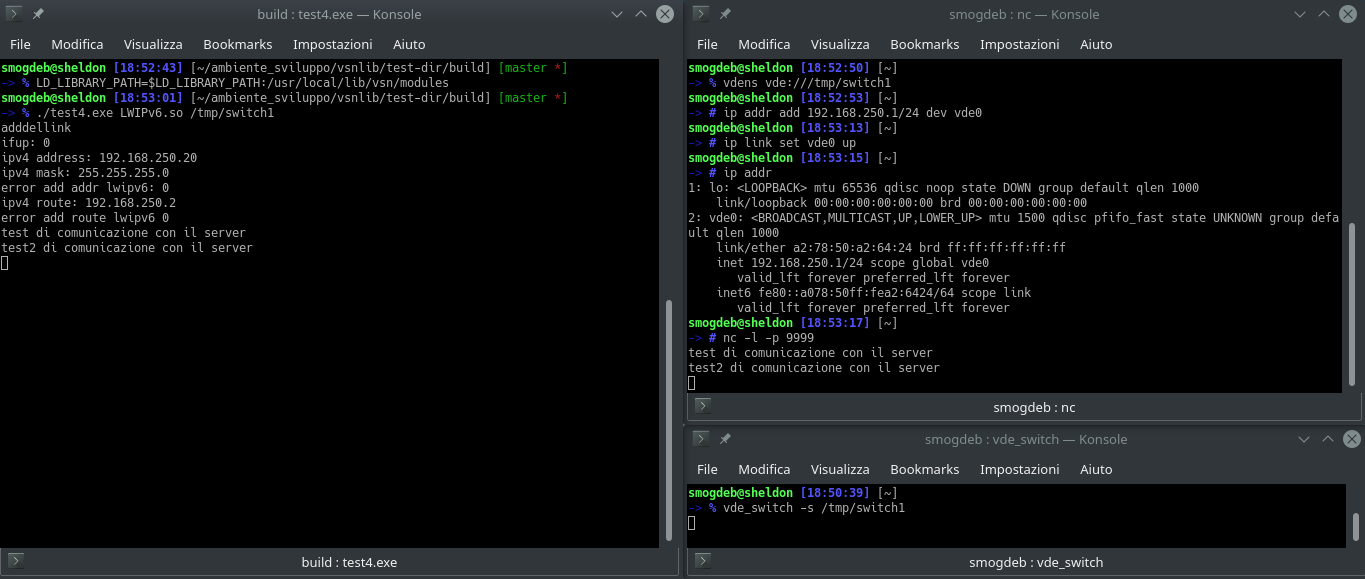
\includegraphics[width=14cm]{test4}%inserisce una figura larga 5cm
                                        %se si vuole usare va scommentata
%
%%%%%%%%%%%%%%%%%%%%%%%%%%%%%%%%%%%%%%%%%inserisce la legenda ed etichetta
                                        %   la figura con \label{fig:prima}
\caption[netcat IPv4]{netcat IPv4}\label{fig:test4}
\end{center}
\end{figure}
\begin{figure}[h]                       %crea l'ambiente figura; [h] sta
                                        %   per here, cio� la figura va qui
\begin{center}                          %centra nel mezzo della pagina
                                        %   la figura
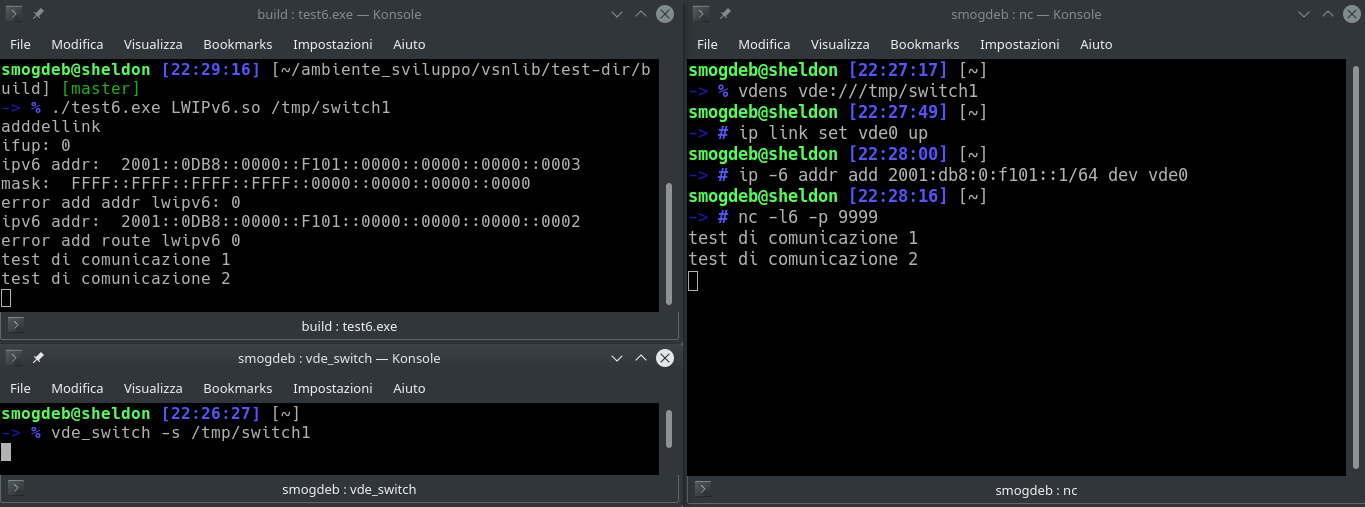
\includegraphics[width=14cm]{test6}%inserisce una figura larga 5cm
                                        %se si vuole usare va scommentata
%
%%%%%%%%%%%%%%%%%%%%%%%%%%%%%%%%%%%%%%%%%inserisce la legenda ed etichetta
                                        %   la figura con \label{fig:prima}
\caption[netcat IPv6]{netcat IPv6}\label{fig:test6}
\end{center}

\end{figure}
\end{itemize}

%%%%%%%%%%%%%%%%%%%%%%%%%%%%%%%%%%%%%%%%%non numera l'ultima pagina sinistra
\clearpage{\pagestyle{empty}\cleardoublepage}
